\chapter{Задача о парковочных местах}

\section{Постановка задачи}
\setstretch{2}

Существует $M$ парковочных мест.

В игре участвуют $N$ игроков, $N >> M$.

$\tilde N$ --- количество севших за руль

$(N - \tilde N)$ --- количество поехавших общественным транспортом.

Издержки игроков $c(x)$:
\begin{itemize}
 \item  $t$, если $\tilde N\le M$,
 \item  $T$, если $\tilde N>M$;
 \item  $\tau$, альтернативный маршрут,
 \item  $t<\tau<T$
\end{itemize}

$\tau$ — альтернативный маршрут.
Сравнить его с лотереей ${t,T}$.
$P(t)$ задается $\tilde N$: $P=\frac{M}{\tilde{N}}$ (or $1$, if $M \le \tilde N$).

\textbf{Чистое равновесие}: $\frac{M}{\tilde N}t+(1-\frac{M}{\tilde{N}})T\approx\tau$.


$\tilde{N}$ (количество севших за руль) : $\frac{M}{\tilde{N}}t+(1-\frac{M}{\tilde{N}})T\le\tau$.

${N-\tilde N}$ (кто едет транспортом) : $\frac{M}{(\tilde{N}+1)}t+(1-\frac{M}{\tilde{N}+1})T\ge\tau$.

$T-\tau = \frac{M}{\tilde{N}}(T-t)$

$\tilde{N}=[\frac{M(T-t)}{T-\tau}]$ — чистое равновесие. Но «так не бывает», ибо неясно, кто эти счастливчики.

$p$ — вероятность сесть за руль.

$Q$[тебе достанется место] такова, что $\tau = Qt+(1-Q)T \Rightarrow Q(T-t)=T-\tau$, $Q*=\frac{T-\tau}{T-t}$.

Но! $Q$ должно быть вычислено как функция от $p$!

\setstretch{2.5}
$(1-p)^{N-1} + \\ (N-1)p(1-p)^{N-2} + \\ C_{N-1}^2 p^2(1-p)^{N-2} + ... + \\ C_{N-1}^{M-1}p^{M-1}(1-p)^{N-M} + \\ C_{N-1}^{M}p^M(1-p)^{N-M-1}(\frac{M}{M+1}) + \\ C_{N-1}^{M+1}p^{M+1}(1-p)^{N-M-2}(\frac{M}{M+2}) + \\ p^{N-1}\frac{M}{N} = \\ Q^*$

Решить как обратную функцию, найти $p^*$ — решение $p^*(\frac{T-\tau}{T-t})$.

\textbf{Гипотеза:} в равновесии $Np^* >> M$.


\section{Подход №2}



$\frac{M}{pN} t + (1 - \frac{M}{pN}) T = \tau$,
что дает
$p=\frac{M(T-t)}{N(T-\tau)}$ в равновесии, если $T$ не зависит от $p$.

А если зависит? Пусть $r = \frac{M}{pN}$

$T = t + f(r)$

$\frac{T-\tau}{T-t} = \frac{M}{pN} = r$, и получаем $(r-1)r(r) = t - \tau$

$1 + \frac{t-\tau}{f(r)} = r$

$f(r)$ --- это потраченное время в зависимости от $r = \frac{M}{pN}$, т. е. от ...?

TODO Начертить график

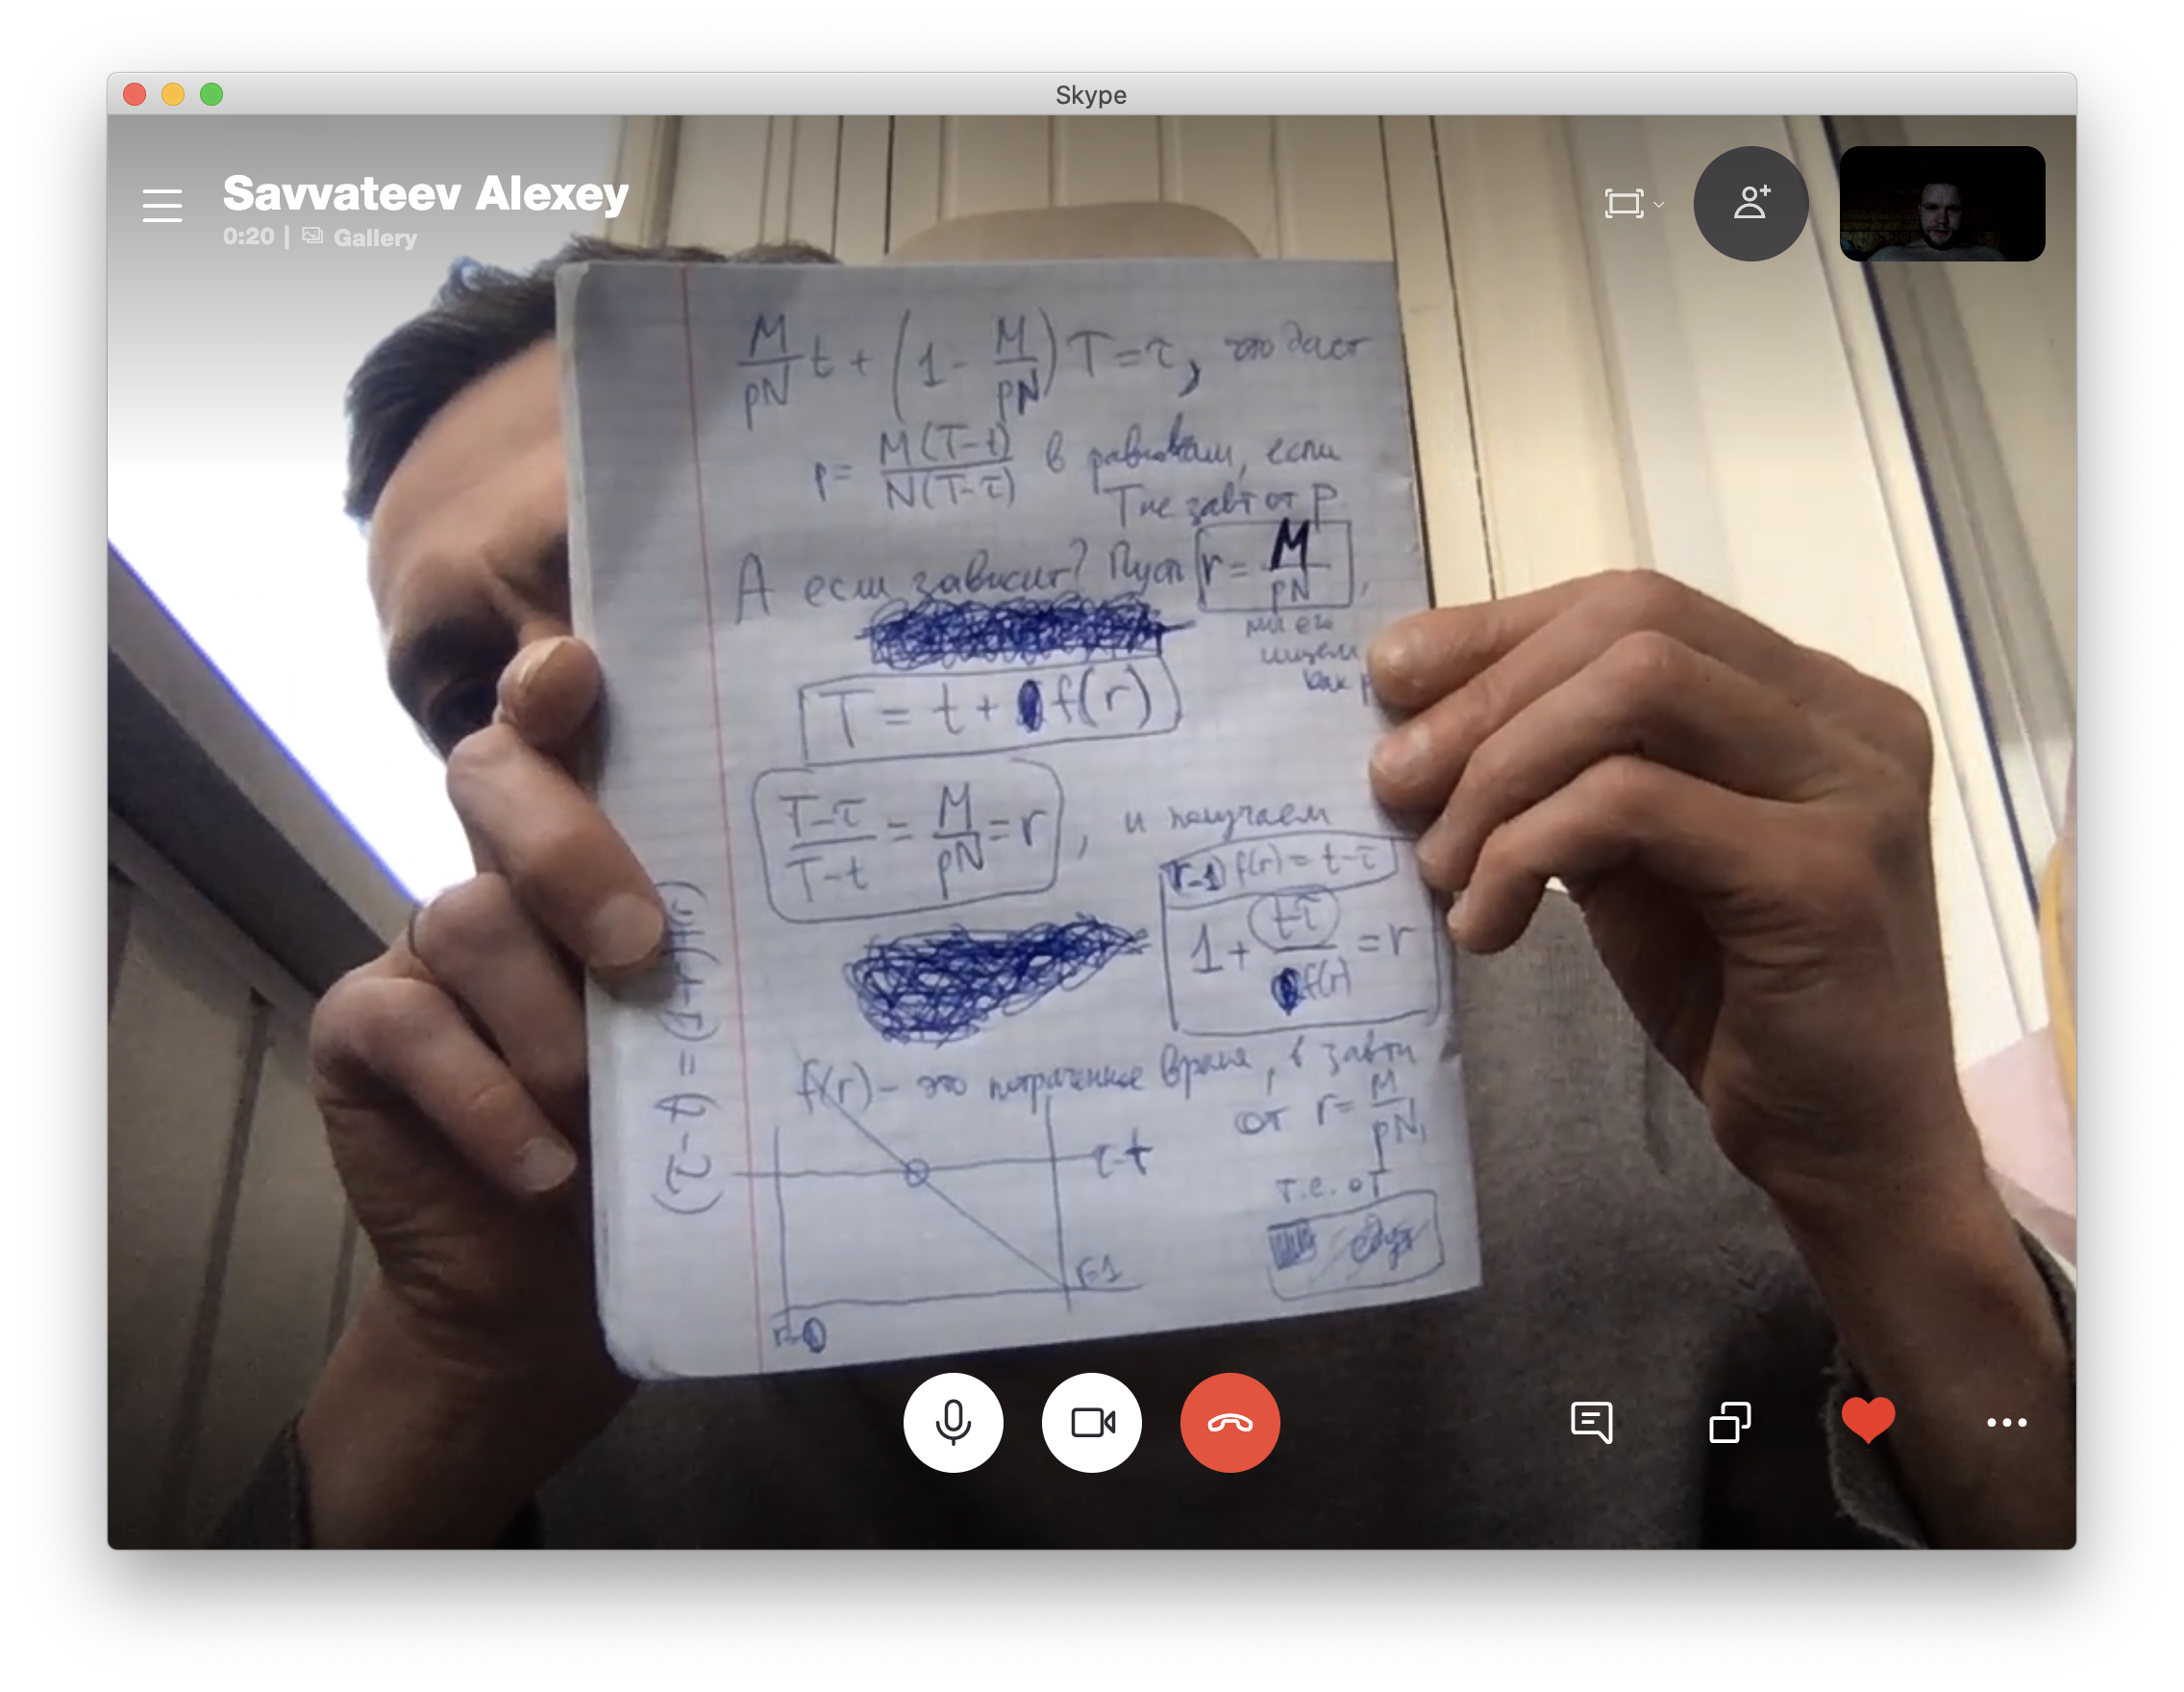
\includegraphics[scale=0.4]{img/tetrad2}
\setstretch{1.2}

\bigskip

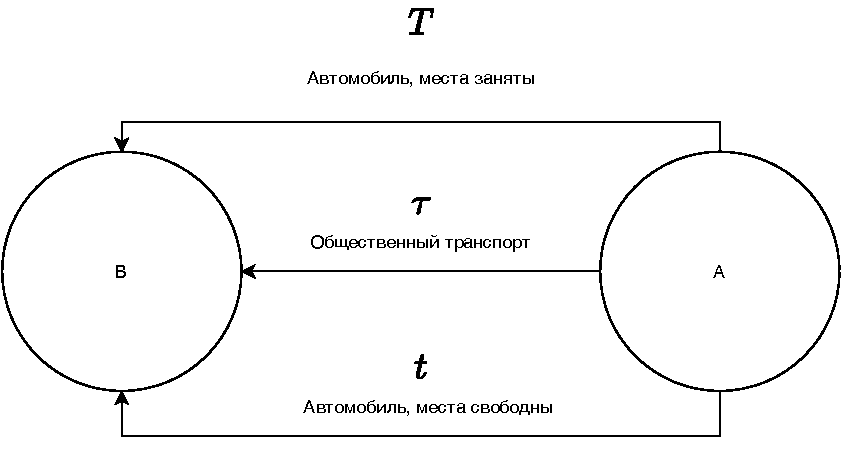
\includegraphics[scale=0.8]{img/task_scheme}


\section{Общее решение}

\inputpython{../code/task1.py}{1}{41}

\subsection{Вариации}

Для $N=1000$:

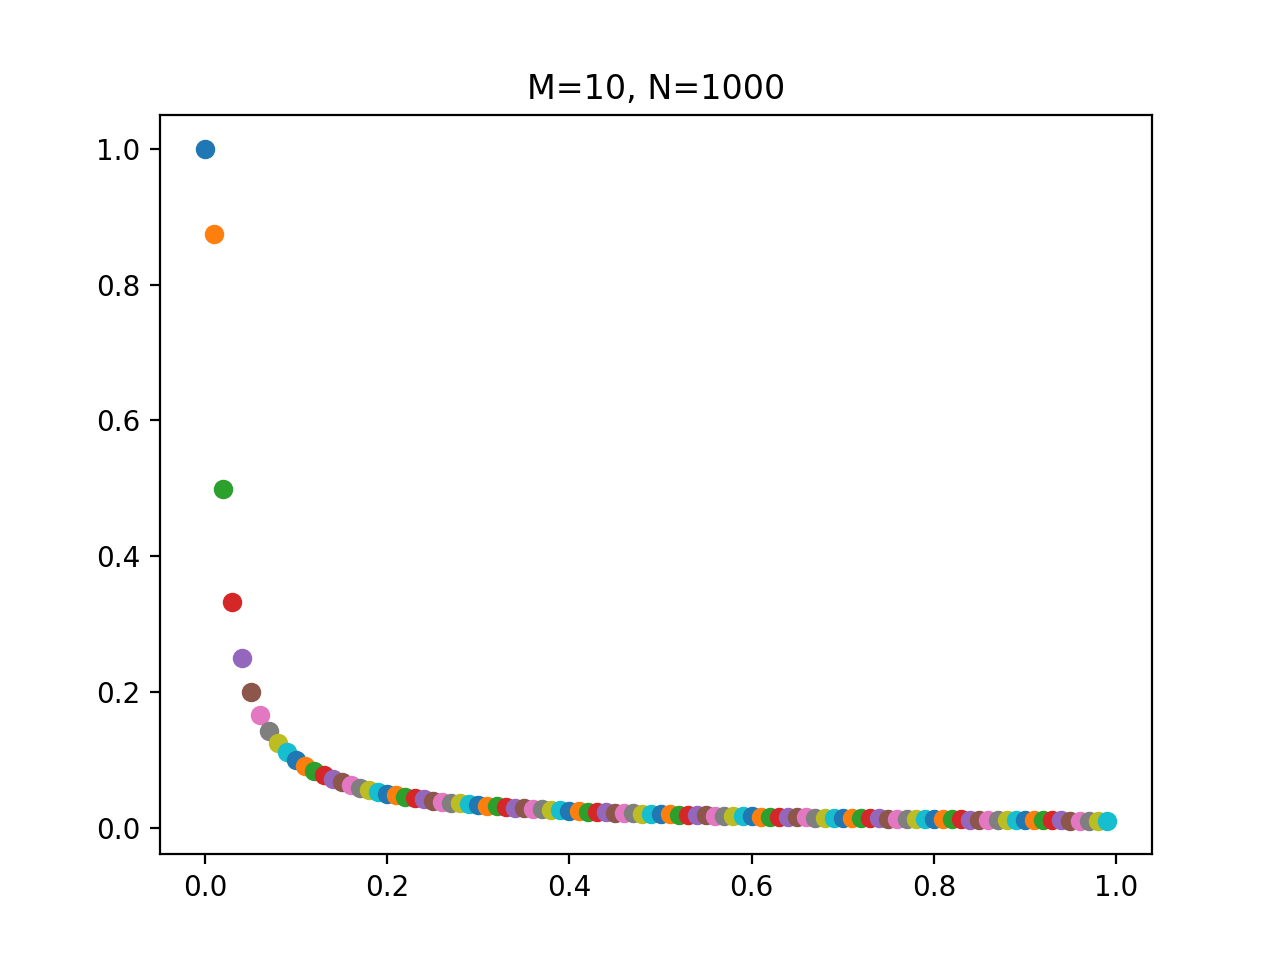
\includegraphics[scale=0.5]{img/1000_10}
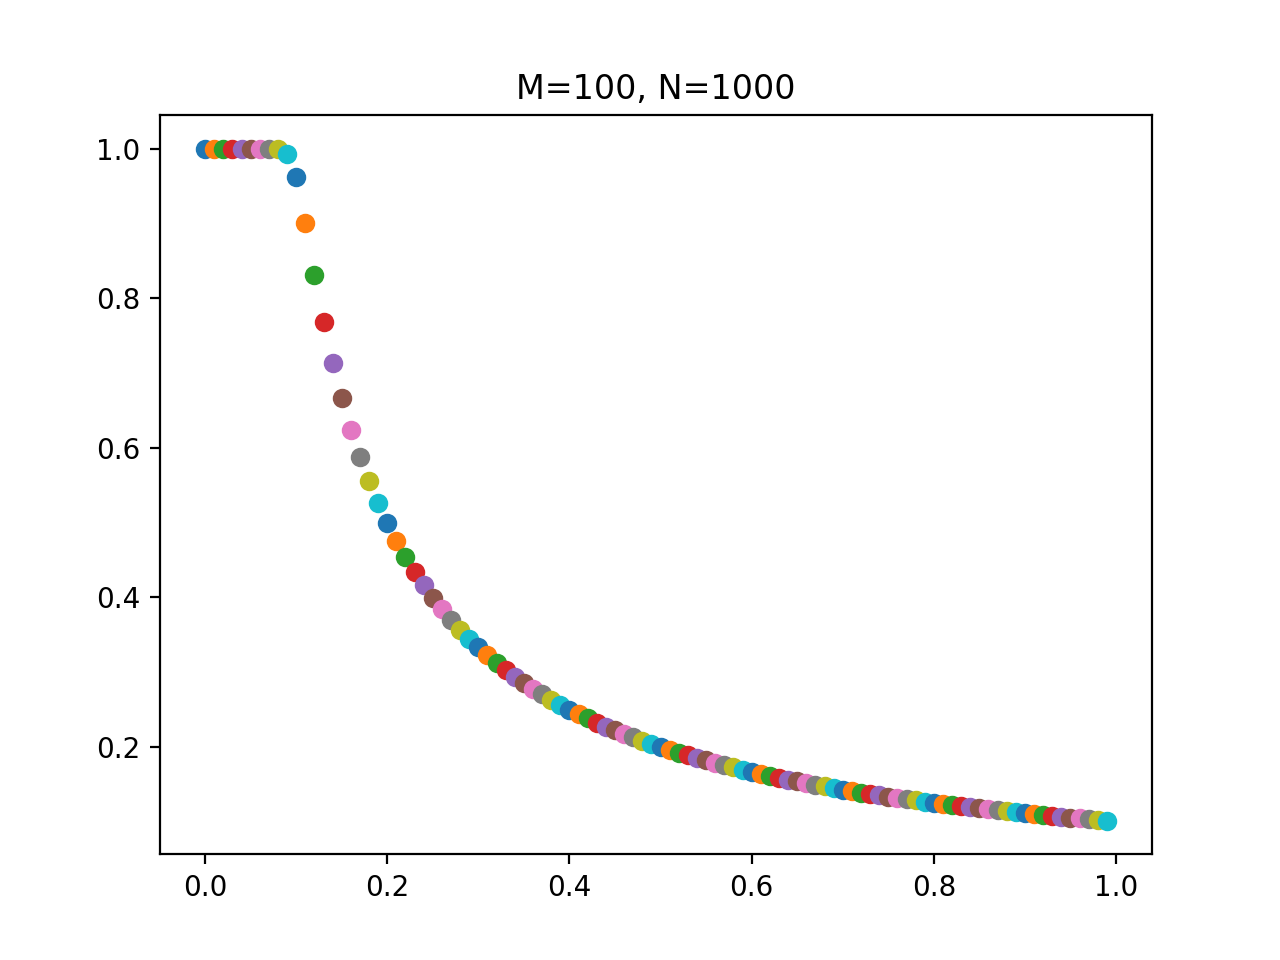
\includegraphics[scale=0.5]{img/1000_100}
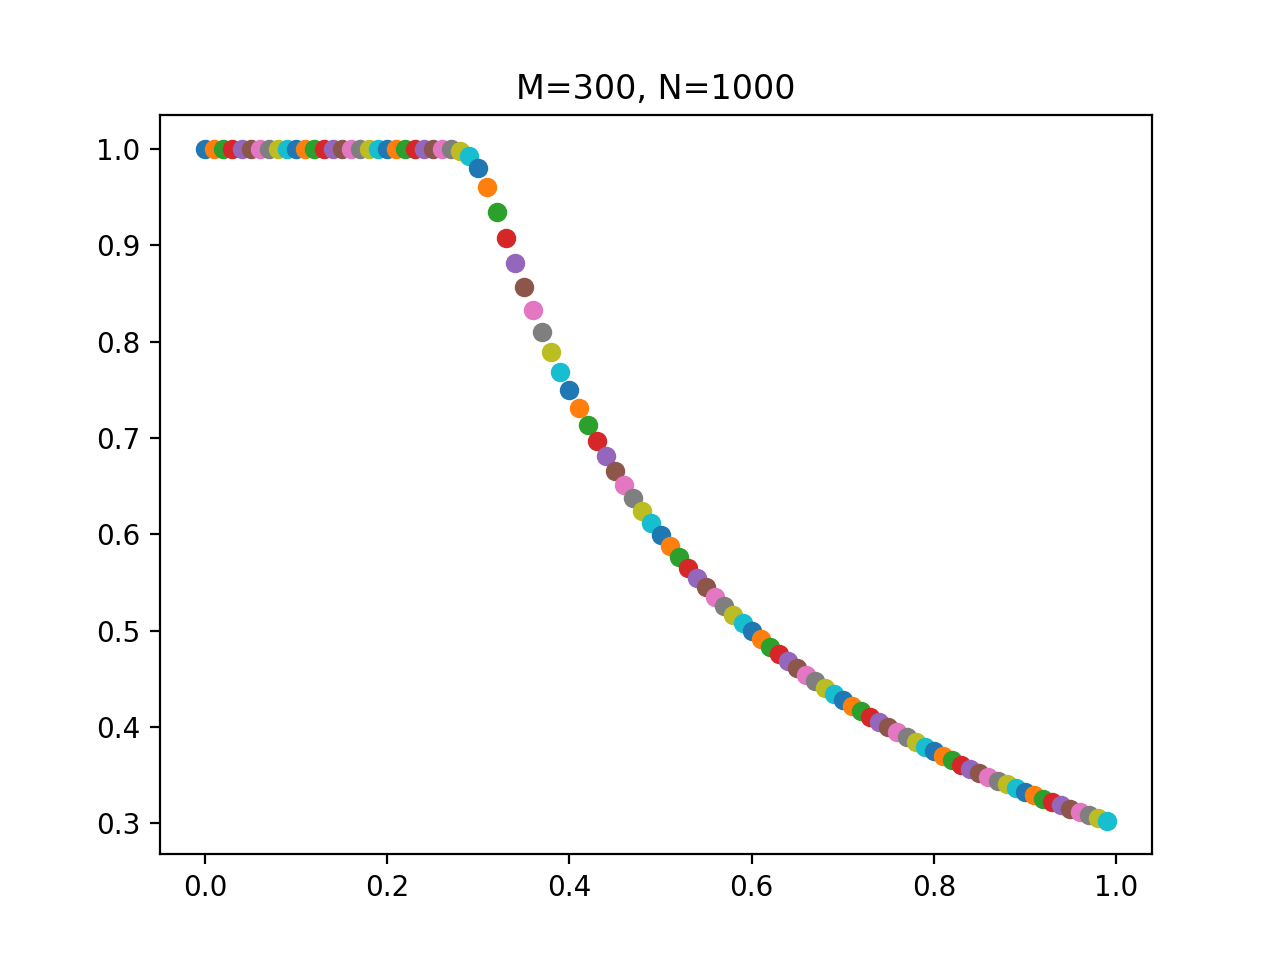
\includegraphics[scale=0.5]{img/1000_300}
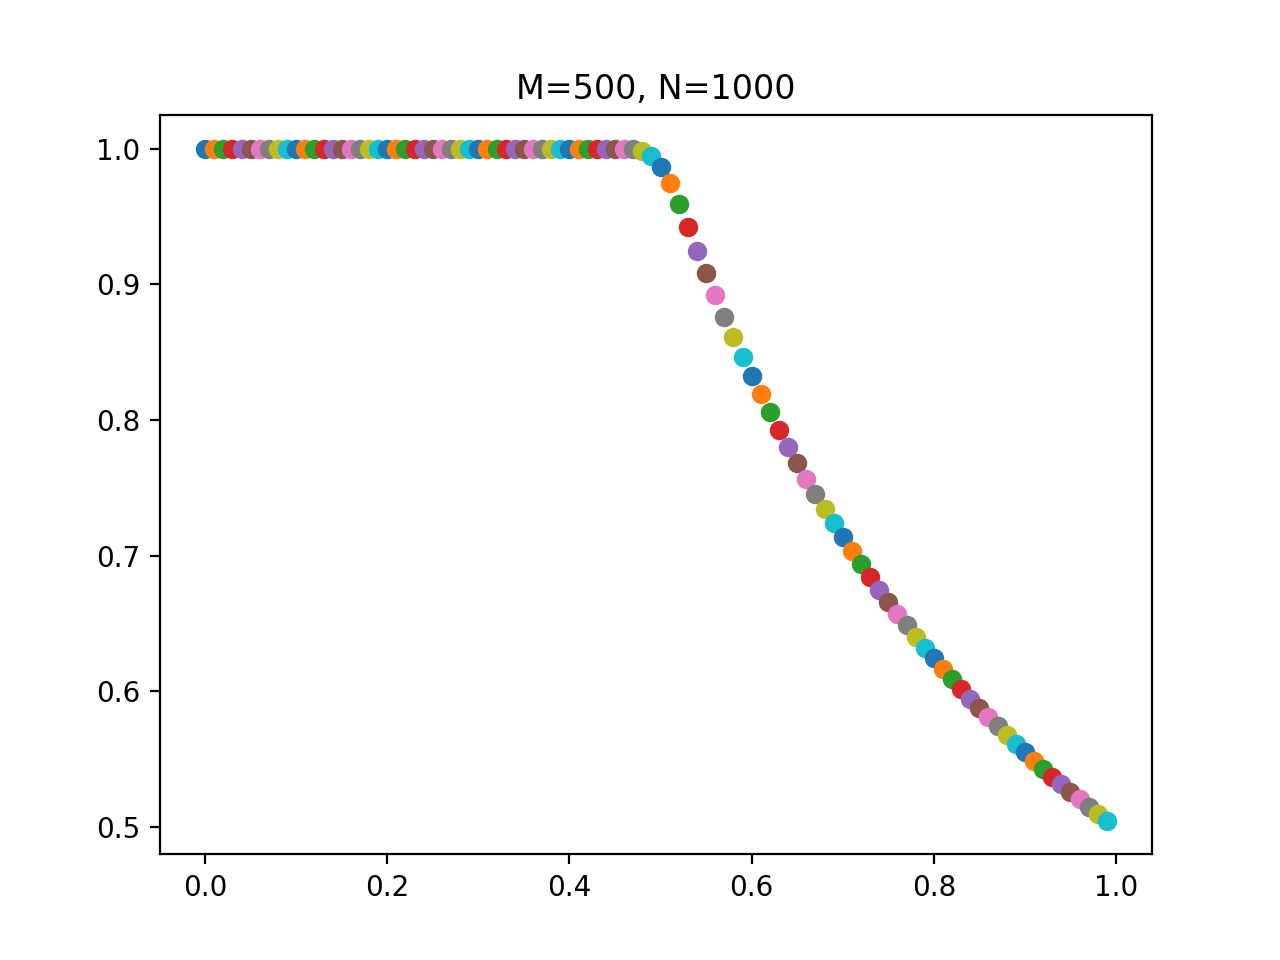
\includegraphics[scale=0.5]{img/1000_500}
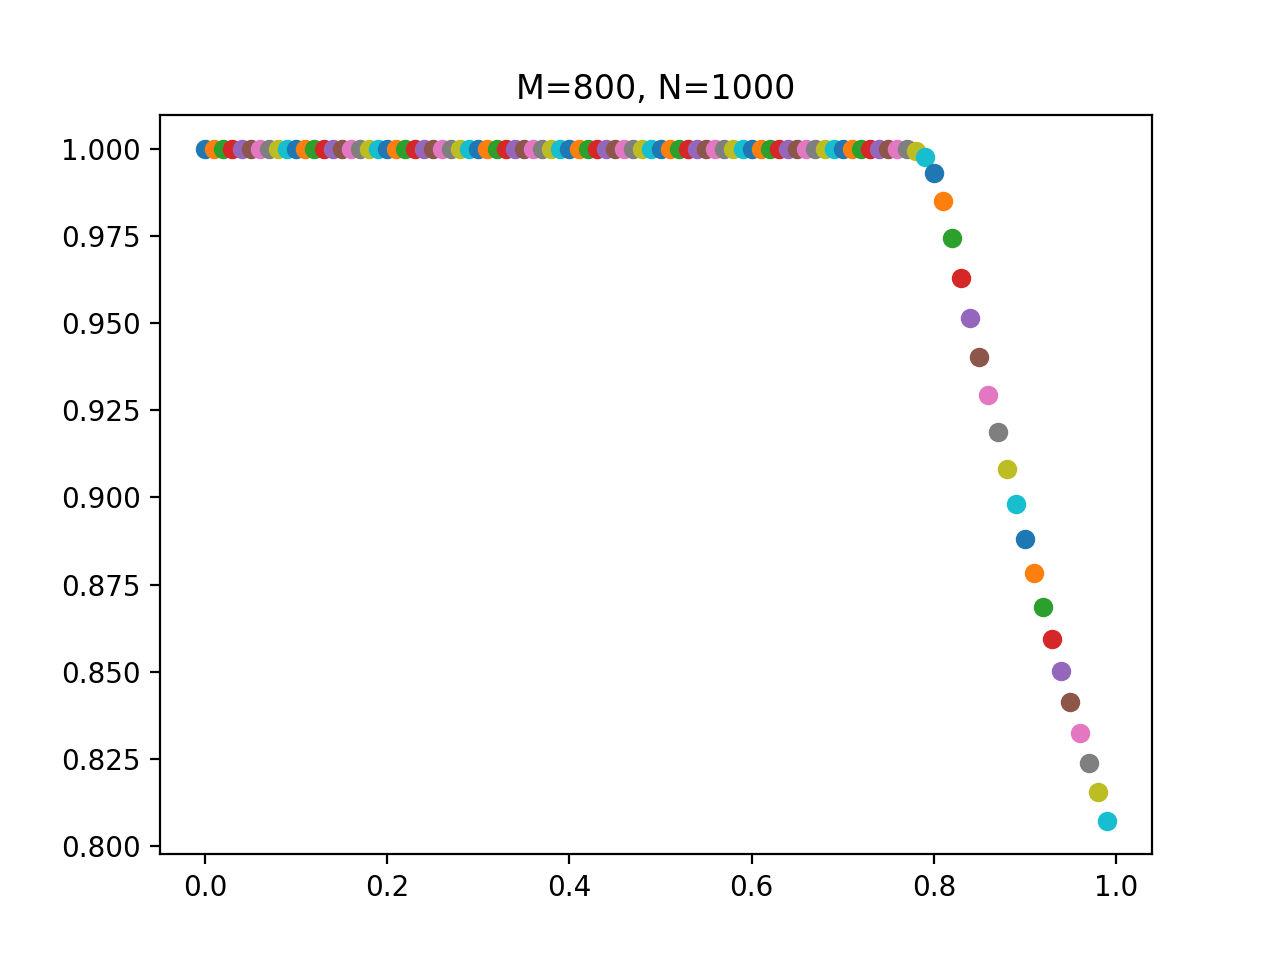
\includegraphics[scale=0.5]{img/1000_800}
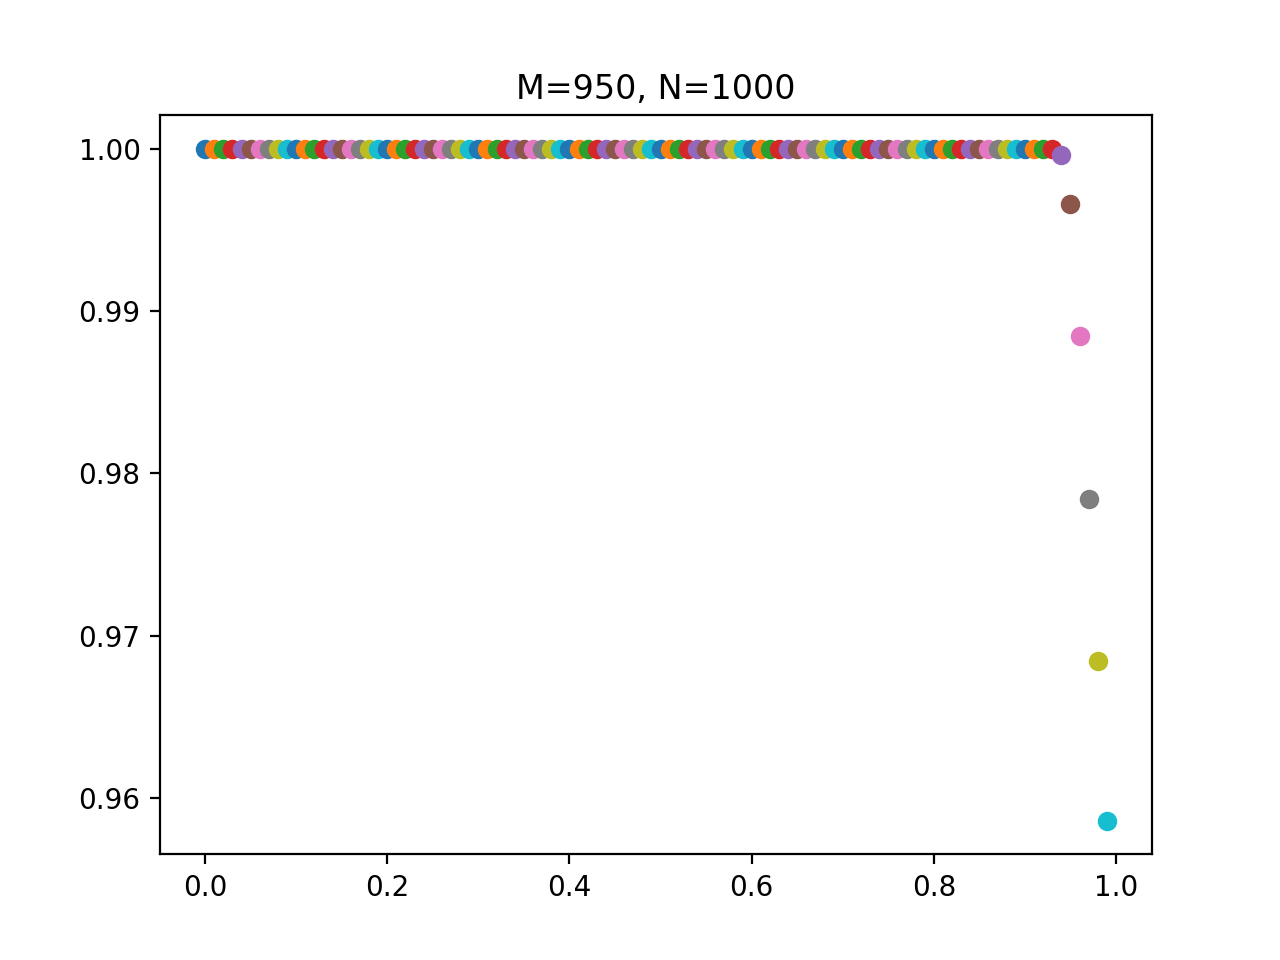
\includegraphics[scale=0.5]{img/1000_950}
\skip
Для $N=100$:

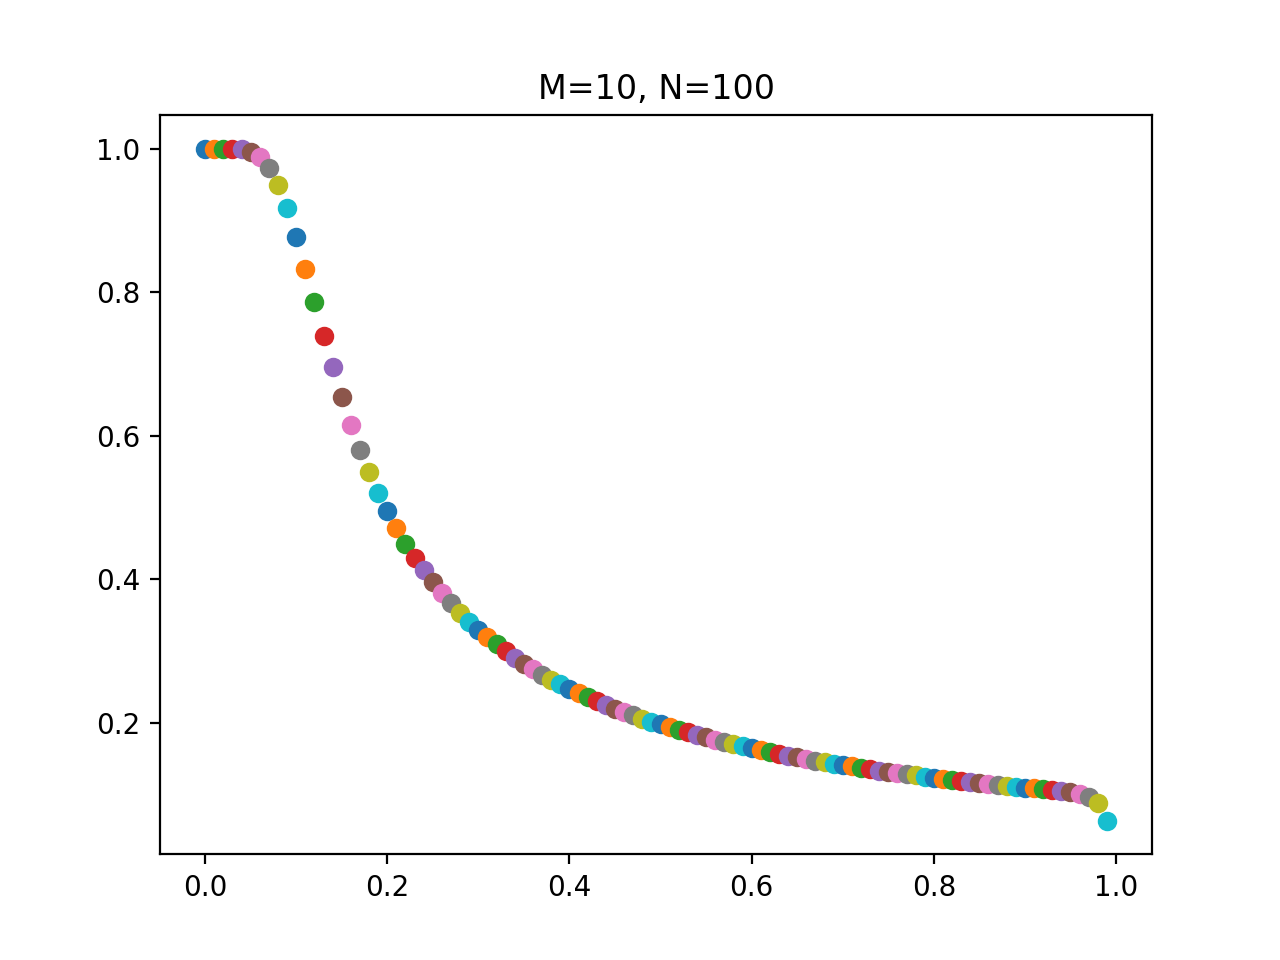
\includegraphics[scale=0.5]{img/100_10}
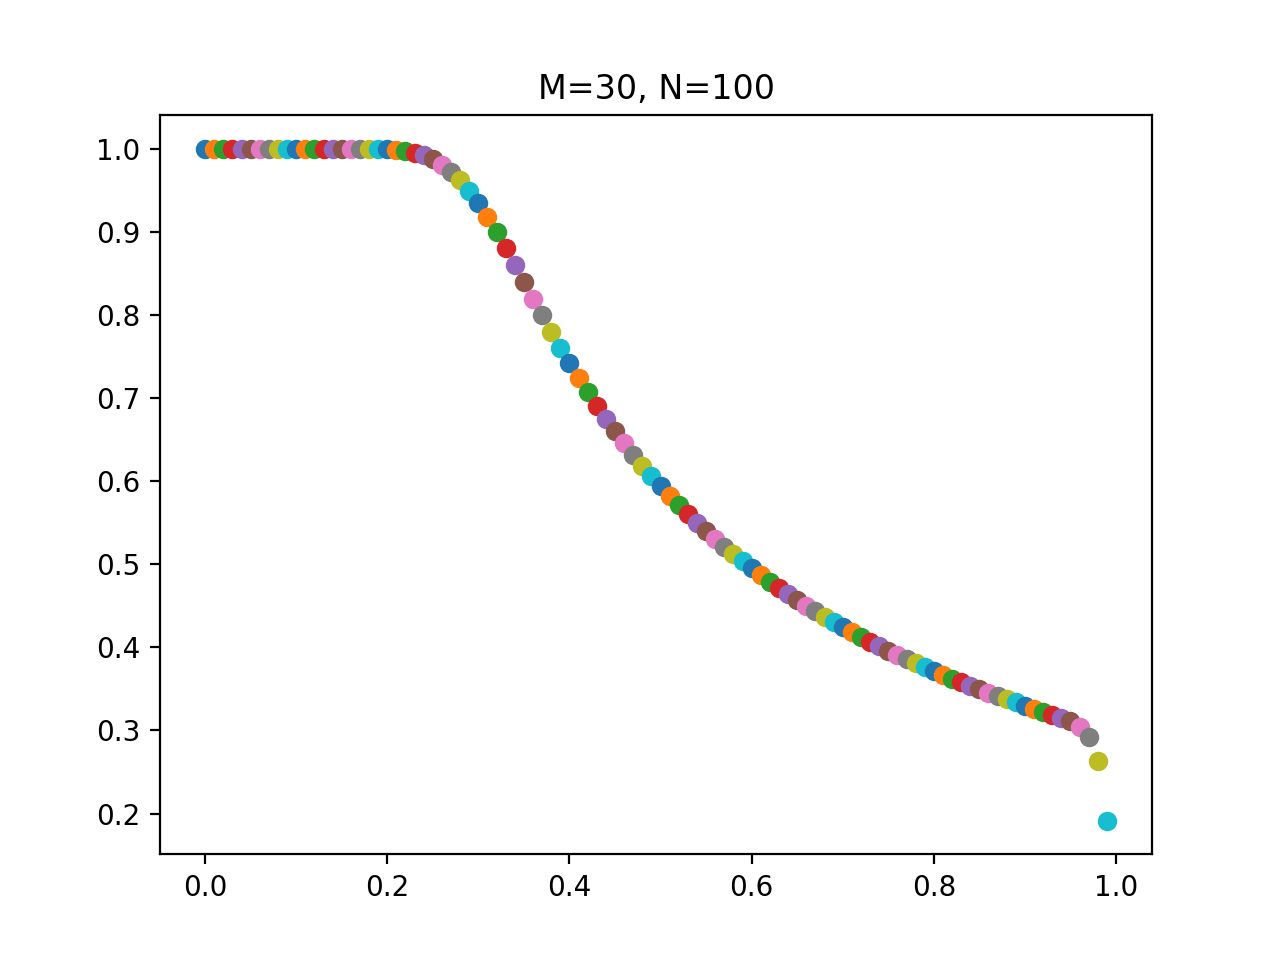
\includegraphics[scale=0.5]{img/100_30}
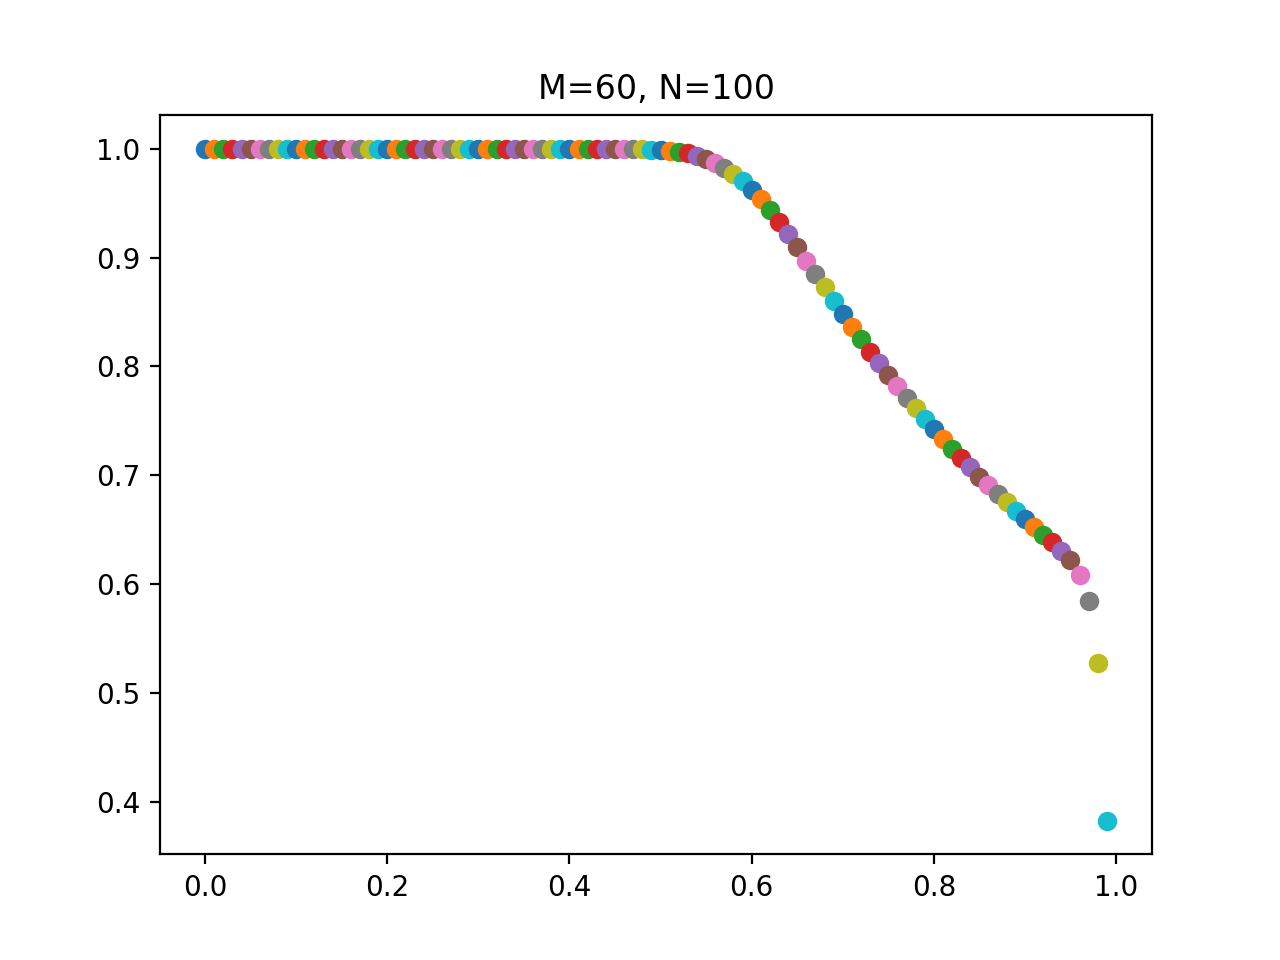
\includegraphics[scale=0.5]{img/100_60}
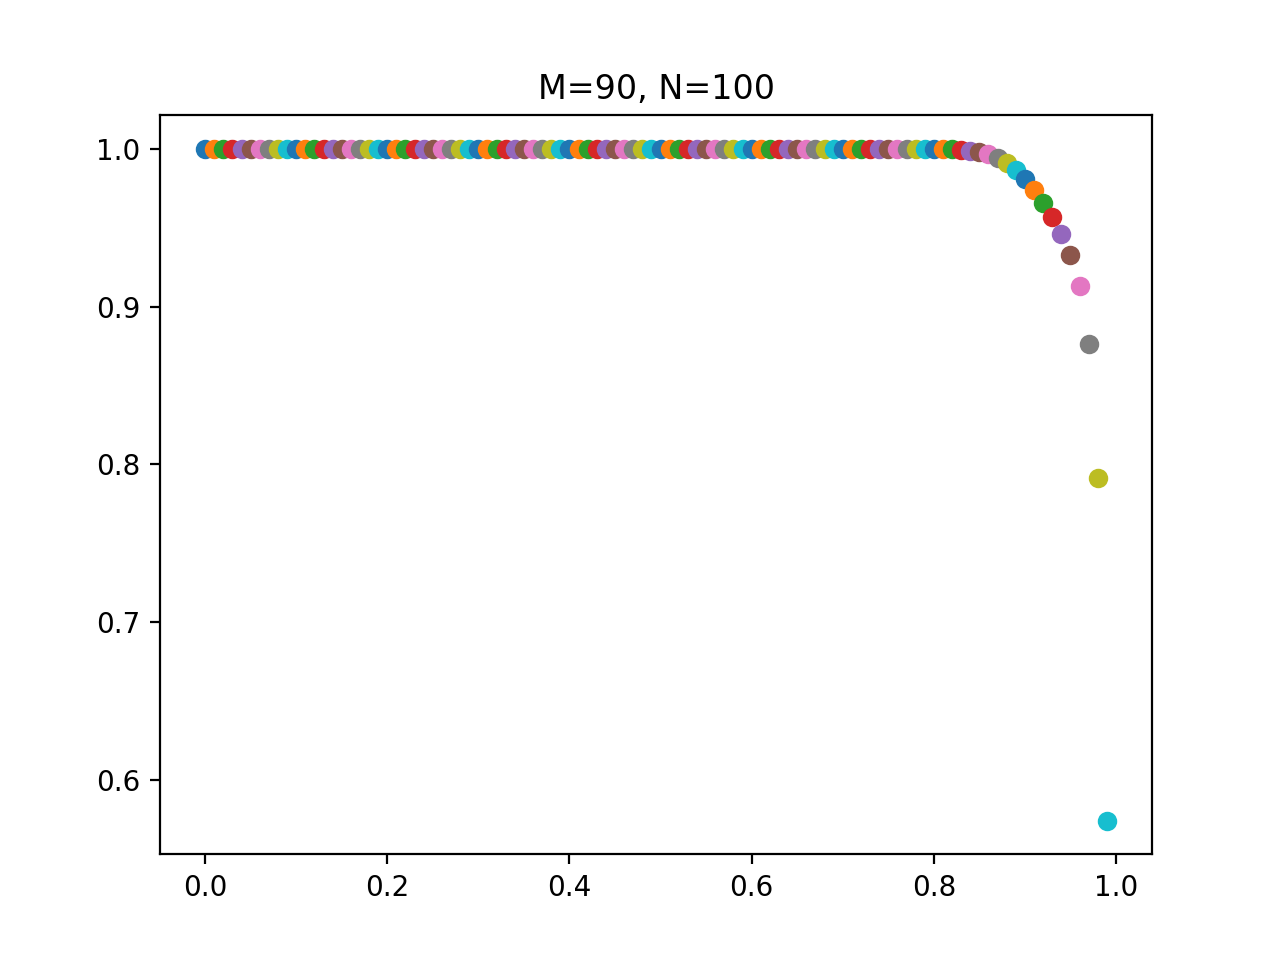
\includegraphics[scale=0.5]{img/100_90}


%\footnote{Предположим, что в Майкоп приехал Николай Басков, и все билеты раскуплены}


%\section{Рассуждения на тему задачи}

\section{Другие подходы к проблеме}
Транспортный поток как физическая материя, состоящая из молекул \cite[168]{lukanin}
\section{Варианты практического решения}
Ценовое регулирование
